\documentclass{comp621}

\usepackage{epsfig} 
\usepackage{alltt}
\usepackage{amsmath}
\usepackage{amssymb}
\usepackage{float}
\usepackage{graphicx}
\usepackage{listings}
\usepackage{multicol}
\usepackage{caption}
\usepackage{url}

\title{Optimizing a robust AspectMATLAB front-end}
\ReportNumber{2016-09}
\author{Hongji Chen}
\date{December 16, 2016}

\captionsetup[lstlisting]{font={small,tt}}
\begin{document}

\MakeTitlePage

\tableofcontents

\listoffigures 
\listoftables 

\clearpage
\section{Introduction and Background}

AspectMATLAB is aimed to provide aspect-oriented programming (AOP) features to
a widely used scientific programming language, MATLAB, which specialized in
matrix computation. However, dynamic features provided by MATLAB, such as
untyped variable, and shared namespace between functions and variables, pose
challenges for transforming and weaving. In the previous two version of
AspectMATLAB, attempts have been made to implement robust transforming
strategies, using the McSAF analysis framework. These approaches are not only
hard to maintain, but also limit the flexibility of the transforming strategies
implementation. Thus, in the project, we purpose a new transforming framework,
sharing similar API interfaces as the previous framework, but providing a more
modular way to implement and assemble the transforming strategies.

\subsection{AspectMATLAB}
AspectMATLAB is an aspect-oriented programming (AOP) implementation in
scientific programming language MATLAB. There has been two previous version of
AspectMALTAB, Toheed Aslam's AspectMatlab compiler \cite{toheed_aspectmatlab},
and Andrew Bodzay's AspectMatlab++ compiler \cite{andrew_aspectmatlb}. The new
AspectMATLAB is built on the success of the two previous version, with
improvement on pattern syntax, pattern validation and argument matching
capability.
 
Since the first version of the AsepctMATLAB, a total of 13 patterns have been
defined. Each of them captures specific type of program points or restricts the
searching scope for the matcher. In the previous two versions of AspectMATLAB,
the compiler doesn't distinguish the type of the patterns. The lack of ability
to verify the patterns, may lead to unexpected behaviours during matching and
weaving. Thus, in the new version of AspectMATLAB, we classify the pattern into
two different sets, the \emph{primitive} patterns and the \emph{modifier}
patterns. The primitive patterns will allow the matcher to select at least one
program point to weave the action code. However, unlike the primitive pattern,
the modifier patterns don't provide any program point, but instead, they
restrict the searching scope of the matcher, and allow matcher to provide more
accurate result. The following table shows each pattern along with its
description and classification.

\begin{table}[!htbp]
\begin{center}
\begin{tabular}{l|l|l}
\hline
Pattern            & Classification & Description                                             \\
\hline
Annotation         & Primitive      & Capture annotation comments                             \\
Call               & Primitive      & Capture function calls                                  \\
Execution          & Primitive      & Capture function execution bodies                       \\
Get                & Primitive      & Capture matrix accesses (read)                          \\
Loop               & Primitive      & Capture whole loop statements                           \\
Loop Body          & Primitive      & Capture loop execution bodies                           \\
Loop Head          & Primitive      & Capture loop head expressions / statements              \\
Main Execution     & Primitive      & Capture the first script / function body that executed  \\
Operator           & Primitive      & Capture arithmetic operation expressions                \\
Set                & Primitive      & Capture matrix accesses (write)                         \\
Scope (within)     & Modifier       & Restrict the searching result by its scope              \\
Shape (dimension)  & Modifier       & Restrict the searching result by its shape              \\
Type  (istype)     & Modifier       & Restrict the searching result by its type               \\
\hline
\end{tabular}
\end{center}
\caption{AspectMATLAB pattern specifiction}
\end{table}


An new pattern type analysis have been developed in the new AspectMATLAB to
statically classify a given compound pattern. If the programmer provide a
pattern with no actual join point selection (i.e. a modifier compound pattern),
instead of blindly accept it, the new AspectMATLAB compiler will mark it as an
error, and then terminate the compilation process. Other than pattern
validation, the new AspectMATLAB change the syntax for several patterns in
order to accommodate the changes in argument matching strategies, and allow
programmer to write more clear patterns. The following table shows the modified
pattern syntaxes in the new AspectMATLAB, along with its syntax in the two
previous versions.

\begin{table}[!htbp]
\begin{center}
\begin{tabular}{l|l|l}
\hline
Pattern    &    Previous Syntax                                                & Updated Syntax                                                                                                     \\
\hline
Get        &    get($\langle$ identifier $\rangle$)                            & get($\langle$ identifier $\rangle$:[$\langle$ shape $\rangle$]$\langle$ type $\rangle$)                            \\
Set        &    set($\langle$ identifier $\rangle$)                            & set($\langle$ identifier $\rangle$:[$\langle$ shape $\rangle$]$\langle$ type $\rangle$)                            \\
Call       &    call($\langle$ identifier $\rangle$:[$\star$,]*[$\dots$])      & call($\langle$ identifier $\rangle$:[$\star$, $\dots$, [$\langle$ shape $\rangle$]$\langle$ type $\rangle$]*)      \\
Execution  &    execution($\langle$ identifier $\rangle$:[$\star$,]*[$\dots$]) & execution($\langle$ identifier $\rangle$:[$\star$, $\dots$, [$\langle$ shape $\rangle$]$\langle$ type $\rangle$]*) \\
Loop       &    loop($\langle$ identifier $\rangle$)                           & loop([for, while, $\star$]:$\langle$ identifier $\rangle$)                                                         \\
Loop Head  &    loophead($\langle$ identifier $\rangle$)                       & loophead([for, while, $\star$]:$\langle$ identifier $\rangle$)                                                     \\
Loop Body  &    loopbody($\langle$ identifier $\rangle$)                       & loopbody([for, while, $\star$]:$\langle$ identifier $\rangle$)                                                     \\
\hline
\end{tabular}
\end{center}
\caption{Updated Pattern Syntax}
\end{table}


\subsection{AspectMATLAB Compiler Structure}
In general, the AspectMATLAB compiler consists of a lexer, a parser, a matcher
and a weaver. \textbf{Lexer} splits the source file character stream into
tokens. \textbf{Parser} assembles the tokens into an abstract syntax tree.
\textbf{Matcher} will traverse the AST tree, and mark all the possible points
for inject the action code, and \textbf{weaver} will apply appropriate
modification to the AST.

In the previous two version of AspectMATLAB, attempts have been made, but not
in a modular way. The following figure shows the general compiler structure of
two previous version.

\begin{figure}[!htbp]
    \begin{center}
    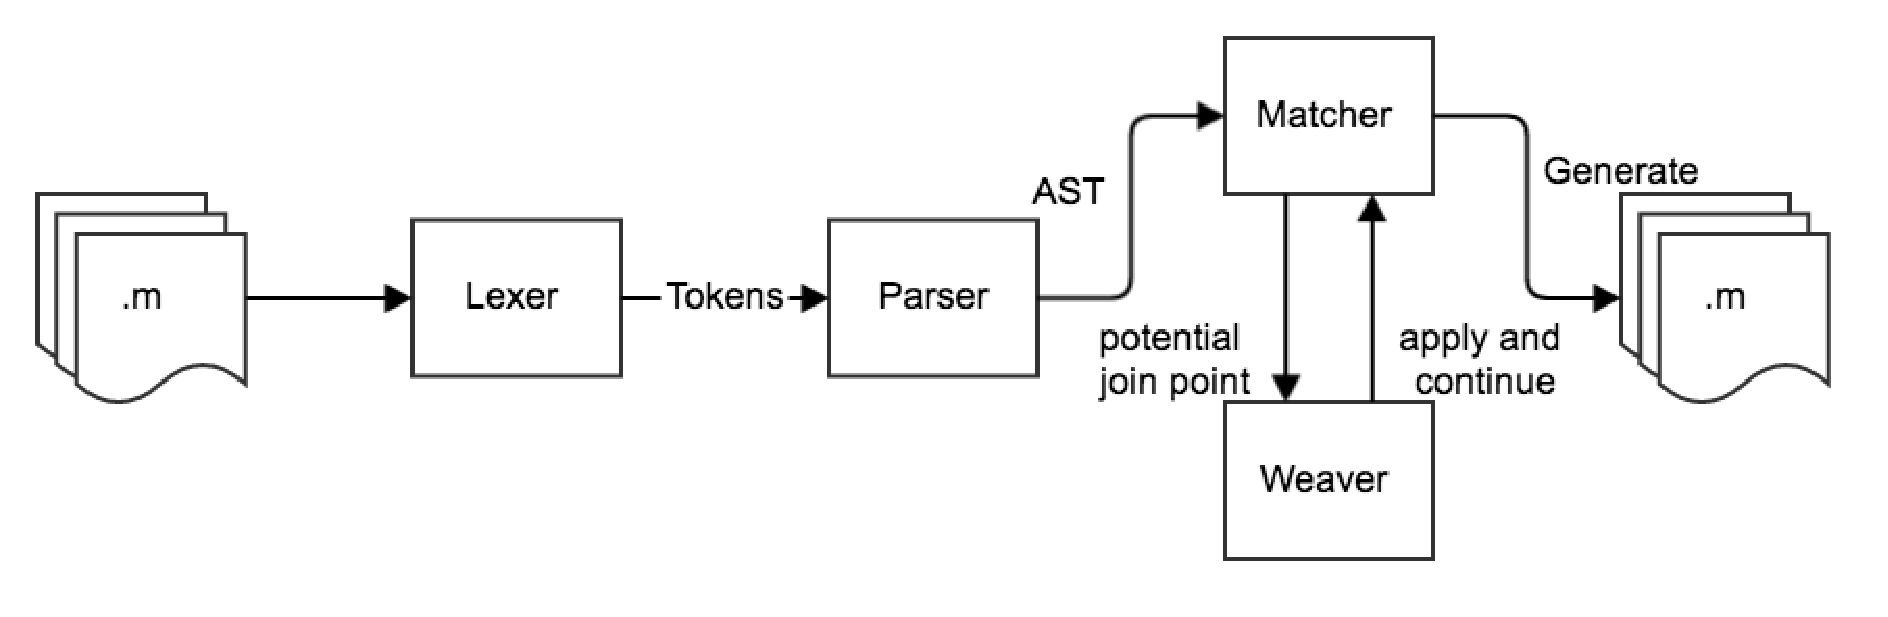
\includegraphics[width=0.9\textwidth]{figures/previous_compiler_structure}
    \end{center}
    \caption{Previous AspectMATLAB compiler structure}
\end{figure}

As shown in the figure, the previous two version of AspectMATLAB actually not
implement the matcher and weaver separately. Instead, every time when a matcher
find a potential join point within the AST, it will call the weaver directly.
In the first version of the AspectMATLAB (Toheed Aslam's AspectMATLAB
compiler), this implementation is proved to be simple and effective. But, when
the scale of the compiler grows larger, this implementation result in
incomplete or even incorrect AST transformation. For example, in the second
version of Aspect MATLAB (Andrew Bo dzay's AspectMATLAB++ compiler), this
implementation leads to duplicate weaving,
\begin{multicols}{2}

\lstinputlisting[language=MATLAB, basicstyle=\footnotesize, numbers=left]
                {codes/duplicateWeave/dw.m}

\end{multicols}

The above aspect will attempt to insert an action before each variable access,
and before each arithmetic addition. Hence, when apply to the following target
code, we should only expect the matrix $x1$, and a arithmetic addition to be
captured.


\lstinputlisting[language=MATLAB, basicstyle=\footnotesize, numbers=left,
                caption={target.m}]
                {codes/duplicateWeave/target.m}
\begin{multicols}{2}
\lstinputlisting[language=MATLAB, basicstyle=\footnotesize, numbers=left,
                caption={generated weaved code}]
                {codes/duplicateWeave/weaved/target.m}
                
\columnbreak
\lstinputlisting[language=MATLAB, basicstyle=\footnotesize, numbers=left,
                caption={expected weaved code}]
                {codes/duplicateWeave/weaved/target_correct.m}
\end{multicols}

As we can see in the above generated weave code, the variable $AM\_tmpBE\_0$,
which is a temporary variable introduced when perform the operator expression
transformation, is identified as a variable access. In order to address these
problems, the compiler structure of the new AspectMATLAB has been modified. The
following figure shows the general compiler structure of the new version.

\begin{figure}[!htbp]
    \begin{center}
    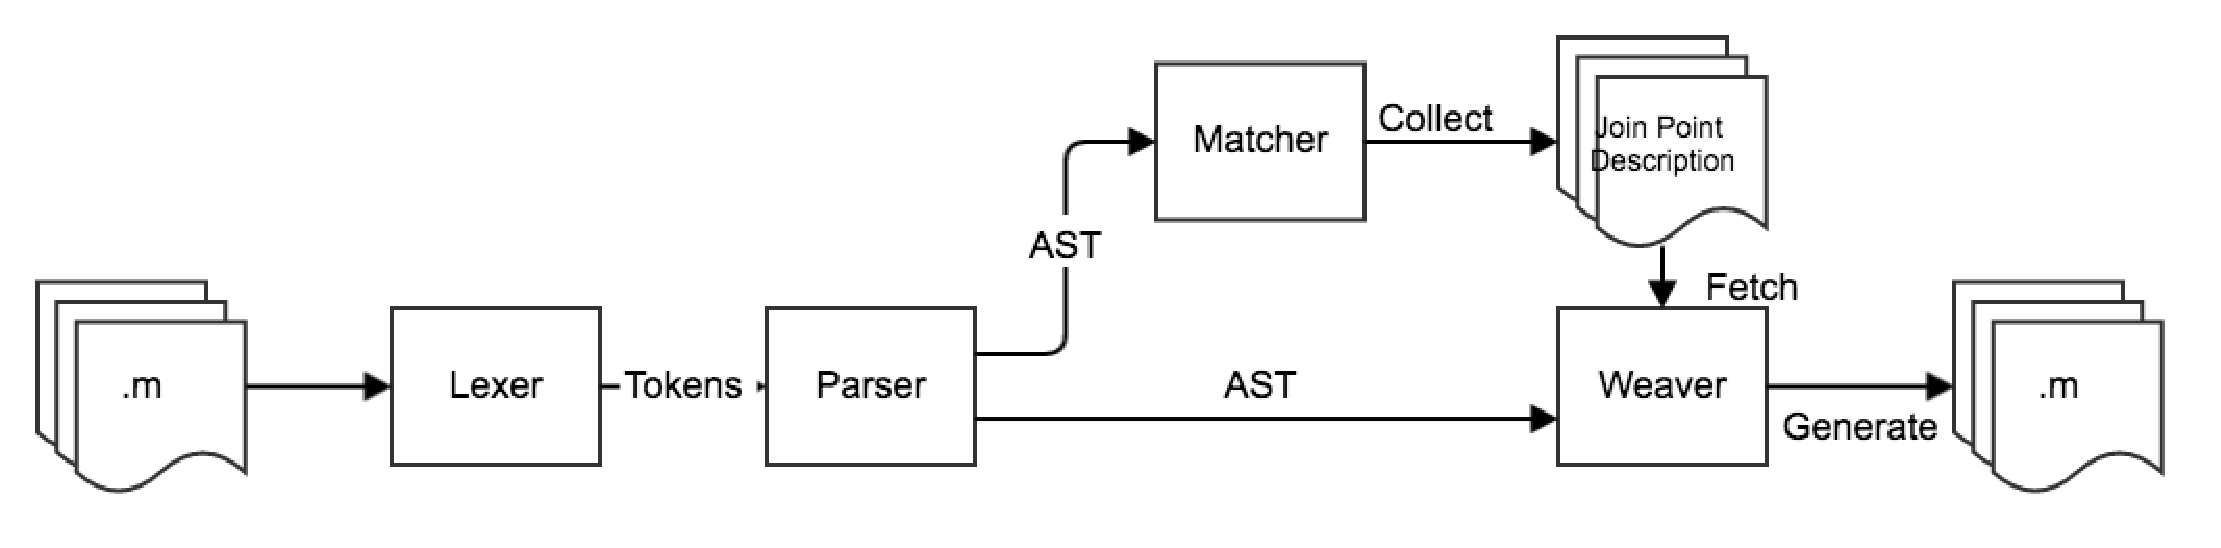
\includegraphics[width=0.9\textwidth]{figures/new_compiler_strucutre}
    \end{center}
    \caption{New AspectMATLAB compiler structure}
\end{figure}

In the new AspectMATLAB compiler, we separate the design of the matcher and the
weaver. Unlike the previous two version of AspectMATLAB which the matching and
weaving are implemented in one pass, the new version has them implemented in
two separate passes. The matching pass communicates with the weaving pass
through a set of objects called `Join Point Descriptions'. A `Join Point
Descriptions' is triple consists of a AST node (i.e. where to insert the code),
 a action node (i.e. which action to apply), and the type of the join point
(i.e. which weaving strategy to apply). The matcher is responsible for 
traversing through the AST, collecting potential join points, apply
then appropriate transforming policy, and then enveloping the join point
information in to a `Join Point Description' object. On the other hand, the
weaver is responsible for fetching `Join Point Description' object, and then
apply the appropriate weaving policy.

As we have described in previous section, a robust transformation and weaving
framework is a vital part to a robust AspectMATLAB compiler. In the previous
two version of AspectMATLAB, the transformation framework is built on the McSAF
analysis framework \cite{mcsaf_master_essay}. McSAF analysis framework is
designed to be a static analysis framework instead of a AST node transforming
framework. Thus, its difficult to implement a transformation using McSAF in an
elegant way. Moreover, in some cases we would like to implement a in-place
transformation (i.e. modify the AST node directly in the original AST). This
result in potential faults in AST transverse. Thus, a new transforming
framework has been introduced in the new AspectMATLAB compiler.

\section{AspectMATLAB Transforming Framework}
In order to address the problems we had in the previous two version of
AspectMATLAB, a new transforming framework is developed. The new transforming
framework shares a similar interface with the previous one. Thus the code can
be easily merged to the new transforming framework. Further, the new
transforming framework utilizes the generic type-safe check provided by the
Java compiler, to enforce the behaviour of the transforming implementation. The
new AspectMATLAB transforming framework is also designed in a modular way. The
programmer can implement each part of the transformer separately, and then
assemble them. The transforming framework consists of three parts -
\emph{expression transformer}, \emph{statement transformer}, and \emph{program
transformer}. Further, the new AspectMATLAB framework defines two types of
transformer - \emph{in-place transformer} and \emph{copy transformer}. The
in-place transformer is expected to apply the transformation on the AST
directly, while the copy the transformer does not modified the original AST,
instead, they return a copy of transformed AST. 

\subsection{Expression Transformer} 
The expression transformer is responsible to apply the transforming policy onto
expressions. There are two types of expression transformer - \emph{in-place
expression transformer} and \emph{copy expression transformer}. The following
figure shows the structure the expression transformer.

\begin{figure}[!htbp]
    \begin{center}
    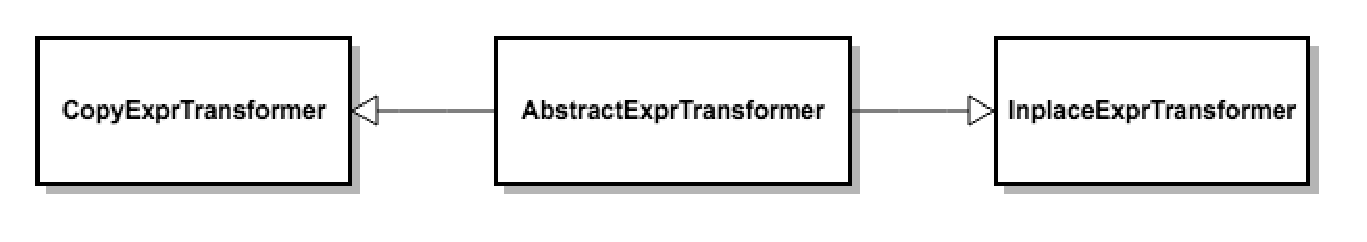
\includegraphics[width=0.9\textwidth]
                    {figures/expression_transformer_structure}
    \end{center}
    \caption{Expression Transformer Structure}
\end{figure}

The \emph{CopyExprTransformer} is an implementation of copy transformer on
expression transformer, and \emph{InplaceExprTransformer} is an implementation
of in-place transformer on expression transformer. Similar to previous
transformer framework, the programmer can modified the behaviour of the
transformer by override the methods associate the specific kind of the
expression. By contract, when programmers extend their own version of
\emph{CopyExprTransformer}, the behaviour of the transformer should follows the
specification defined in the copy transformer (i.e. it does not modified on the
AST directly, instead, they return a copy of AST with transformation applied).

In the previous version, each node case handler is a void method, and its the
callee responsibility to assemble the AST list. This makes the implementation
of transformation contains lots of redundant part, and even lead to potential
faults in the new implementation. Thus in the new AspectMATLAB transformation,
the responsibility of assembling the transformed expression is taken by the
caller method (i.e. the transformation framework transversing method). In order
to achieve this features, the return value of the AST node handle method, has
been modified from void to \emph{ast.Expr}. The programmer only need to
implement the transformation to the expression and pass the transformed
expression AST node as a return value.

\subsection{Statement Transformer}
Similar to the expression transformer, the statement transformer have two
different versions - \emph{CopyStmtTransformer} and
\emph{InplaceStmtTransformer}. The \emph{CopyStmtTransformer} is an
implementation of copy transformer on statement transformer, and
\emph{InPlaceStmtTransformer} is an implementation of in-place transform on
statement transformer. The following figure shows the structure of the
statement transformer.

\begin{figure}[!htbp]
    \begin{center}
    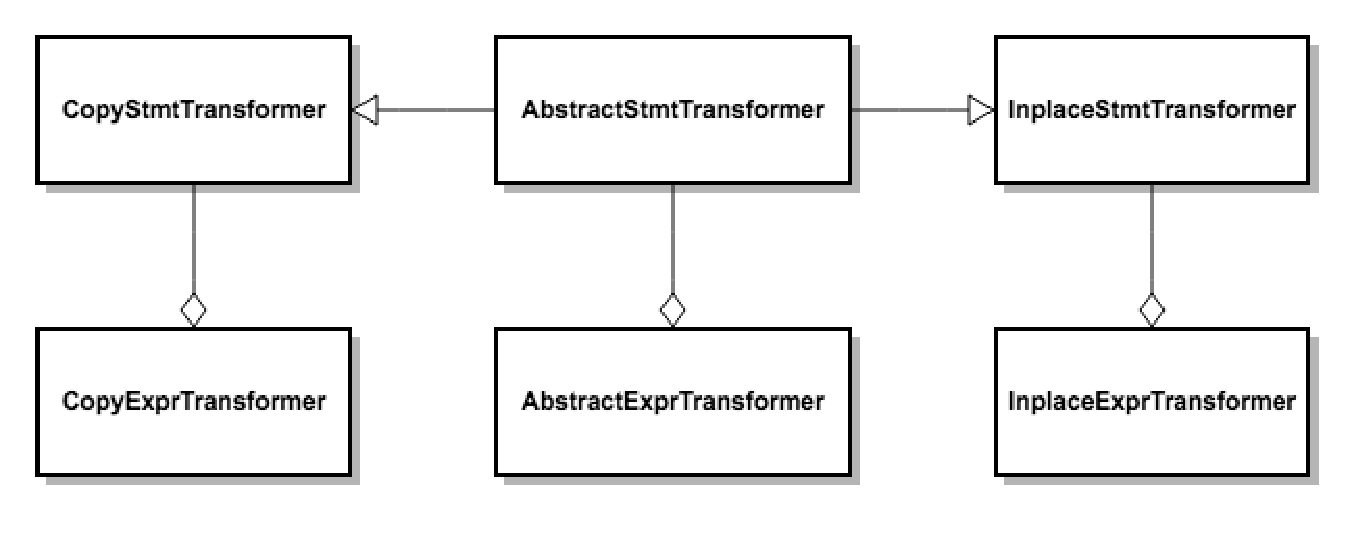
\includegraphics[width=0.9\textwidth]
                    {figures/statement_transformer_structure}
    \end{center}
    \caption{Statement Transformer Structure}
\end{figure}

Each statement transformer consists of a expression transformer. By contract,
this expression transformer should handle all the expression transformation
required by the statement transformer. Once a statement transformer instance is
created, it bind with a expression transformer. Notice that, a copy statement
transformer can only bind with a copy expression transformer, and a in-place
statement transformer can only blind with a in-place expression transformer.
Such rule is imposed by the generic type-safe check by Java. Thus, this make
sure the behaviour of the transformer is consistent (i.e. a in-place statement
transformer will never copy the AST, and a copy state transformer will never
modified the original AST). Here are the signatures of two type of the
statement transformers.

\lstinputlisting[language=Java, basicstyle=\footnotesize, numbers=left,
                 caption={Statement Transformer Signatures}]
                {codes/signatures/StmtTransformerSig.java}

Like the expression transformer, return type of the statement transformer has
been changed from void to \emph{List$\langle$ast.Stmt$\rangle$}. But unlike
the expression transformer, which only allow exactly one expression AST node as
the return value, the statement case handler methods allow a list of statement
AST node. The order of assembling the return value, is exactly the same as the
order of the statement AST node within the list. In this way, the programmer
can implement the transforming strategy that replace one single statement, into
multiple statements. The detailed examples will be covered in the next
section.

\subsection{Program Transformer}

The program transformer represent the hight level of transformation in the
transformer framework. It is responsible for transversing through the
functions, scripts, class definitions and aspect definitions. Every time the
programer transformer encounter a statement, a expression or a
pattern, it will call its internal statement transformer, expression
transformer and pattern transformer respectively. The following figure below
shows the structure of a program transformer, and signatures of program
transformers.

\begin{figure}[!htbp]
    \begin{center}
    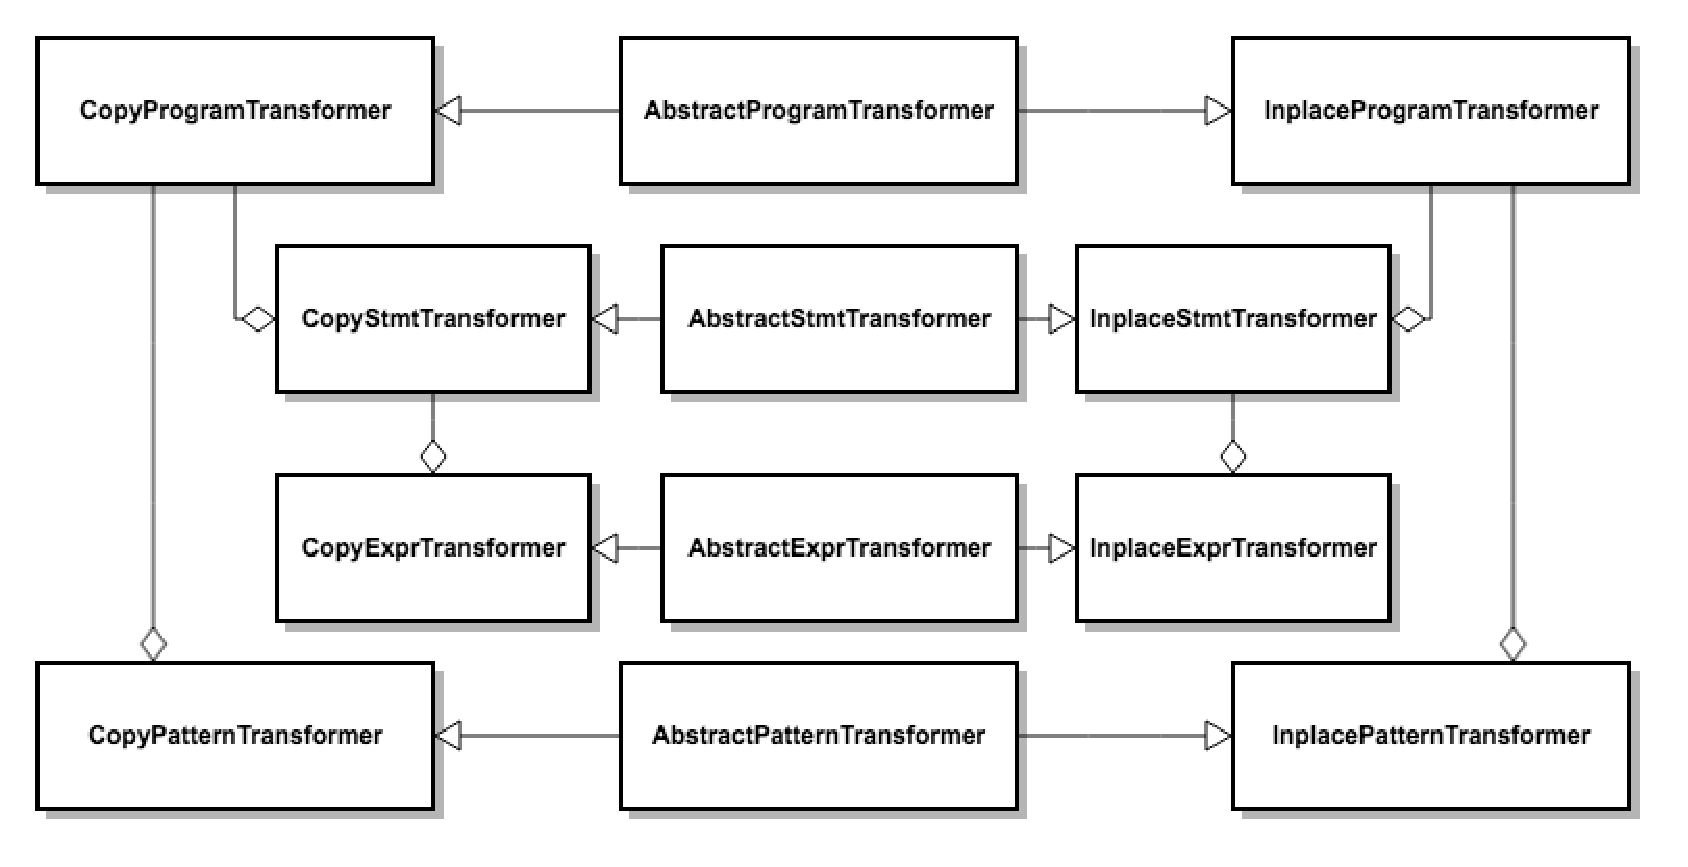
\includegraphics[width=0.9\textwidth]
                    {figures/program_transfomer_structure}
    \end{center}
    \caption{Program Transformer Structure}
\end{figure}

\lstinputlisting[language=Java, basicstyle=\footnotesize, numbers=left,
                 caption={Program Transformer Signatures}]
                {codes/signatures/ProgramTransformerSig.java}

Similar to the statement transformer, the behaviour of the program transformer
is consistent, and such feature is enforced by the Java generic type-safe
check. The return type of the AST node handler methods is also changed from
void to \emph{List$\langle$ast.ASTNode$\rangle$}. The programmer can simply
implement the transformation strategy directly, and let the transformation
framework take care of the assemble process.

\section{Transforming Framework in Action}

In this section, we will go over several example implementation of transforming
policies using the new transforming framework. We will first start with some
small examples, and finally move the the implementation of the aspect matching
transformation.

\subsection{Constant Folding}

The simple example is constant folding. First, we need to decide if we want to
build the transformer as a in-place transformer or a copy transformer. In this
example, we are going to implement this transformer using the copy transformer
as base class. The next step is to decide each component of the transformer, as
in this example, as we are only interested in the expression (i.e. constant
value expression), the only component we need to implement is the expression
transformer, and simply use the trivial statement transformer and program
transformer to assemble the whole transformer.

After we decide which component we need to implement, we need to consider which
AST node case handler method we need to override. In this example, we aimed at
constant folding, so the methods we are going to implement are \emph{PlusExpr},
\emph{MinusExpr}, \emph{MTimesExpr} and \emph{MDivExpr} (to keep this example
simple, we only focus on these four cases). Lets fist see the implementation of
the \emph{PlusExpr},

\lstinputlisting[language=Java, basicstyle=\footnotesize, numbers=left,
                 caption={Constant Folding - Plus Expression}]
                {codes/constant_folding_plus_expr.java}

In the \emph{PlusExpr} AST node case handler method, we first perform the
transformation on the left-hand-side expression and right-hand-side expression 
recursively. Then we check if both expressions are constant integer value
expression. If we we have both side of the expressions are constant integer
value expression, then we perform the addition between the values, and return a
\emph{IntLiteralExpression}, otherwise, we return a copy of the original
expression. In the same manner, we implement other four AST node case handler
methods,

\lstinputlisting[language=Java, basicstyle=\footnotesize, numbers=left,
                 caption={Constant Folding}]
                {codes/ConstantFolding.java}

The transformer above will traverse through the AST and folding the constant
valued integer plus expressions, minus expressions, matrix multiplication
expressions, and matrix division expressions. Let's apply our constant-folding
transformer to a MATLAB script, and here is the result.

\begin{multicols}{2}
\lstinputlisting[language=MATLAB, basicstyle=\footnotesize, numbers=left,
                 caption={Constant Folding Input Script}]
                {codes/constant_folding.in}
\columnbreak
\lstinputlisting[language=MATLAB, basicstyle=\footnotesize, numbers=left,
                 caption={Constant Foling Output Script}]
                {codes/constant_folding.out}
\end{multicols}

\subsection{Statement Execution Tracing}
This example shows the capability of the statement transformer. In Assignment,
we implement a tracing tool using the McSAF framework. In McSAF framework, a
ignore set is required, in order to avoid the recursive transform problem. The
new AspectMATLAB transformer framework provide a more elegant solution. The
responsibility of maintain the ignore set, traverse through the AST in correct
order and assemble the AST, falls on the transform framework.  In this example,
we are going to implement a statement tracing transformer using the in-place
statement transformer.

Let's follow the same steps that we used when design the constant-folding
transformer. First we need to isolate which AST node we need to perform the
transformation. In this case, we need to insert a tracing statement after each
statement. Thus, we need to override the $transform$ method in the in-place
statement transformer.

\lstinputlisting[language=MATLAB, basicstyle=\footnotesize, numbers=left,
                 caption={Statement Tracing Transformer}]
                {codes/StatementTracing.java}

The above transformer will append a $disp$ statement that printing out the type
of AST Node, after each statement in original AST. As this is a in-place
transformer, after we invoke the $transform$ method, all AST modifications are
applied to the original AST. The following are the result that we apply this
transformer to a example program.

\begin{multicols}{2}
\lstinputlisting[language=MATLAB, basicstyle=\footnotesize, numbers=left,
                 caption={Statement Tracing Input}]
                {codes/statement_tracing.in}
\columnbreak
\lstinputlisting[language=MATLAB, basicstyle=\footnotesize, numbers=left,
                 caption={Statement Tracing Output}]
                {codes/statement_tracing.out}    
\end{multicols}

\subsection{Aspect Transformation}
The final example that will given in this report is the AspectMATLAB aspect
transformation. Before weave the action code, we need to apply appropriate
transformation to the AST to make the join point exposed. The new AspectMATLAB
compiler takes the advantage of the modularity of the new transformation
framework. Instead of build all the transformation in a giant class (the
previous approach), we split the implementation of the transformation in to
multiple layers. The first layer is the expression level, this include the
\emph{get}, \emph{set}, \emph{call}, and \emph{operator} patterns. The second
layer is the statement level. This include the \emph{loop}, \emph{loophead},
,\emph{loopbody} and \emph{annotation} pattern. The statement level
transformation is also responsible for injecting the pre-expression statements,
and post-expression statements that generated by the expression level
transformer. The final layer of the transformation framework is the program
level transformer. The program transformer focus on the \emph{execution},
\emph{mainexecution} pattern.

\subsubsection{Expression Level Transformation}
At this level, we focus on each element with the expression, and we generate
two set of statements - the pre-expression statements, and post-expression
statements. During the expression transformation, it is inevitable to generate
temporary variables, and assign values to them. However, this is impossible to
be performed only at expression level. Thus, we add the pre-expression
statements set, and the post-expression statements set. The pre-expression
statements set contains the statements that will be inject just before the
expression, and the post-expression statement set contains the statements that
will be inject just after the expression. The following figure demonstrate the
process of a expression transformer.

\begin{figure}[!htbp]
    \begin{center}
    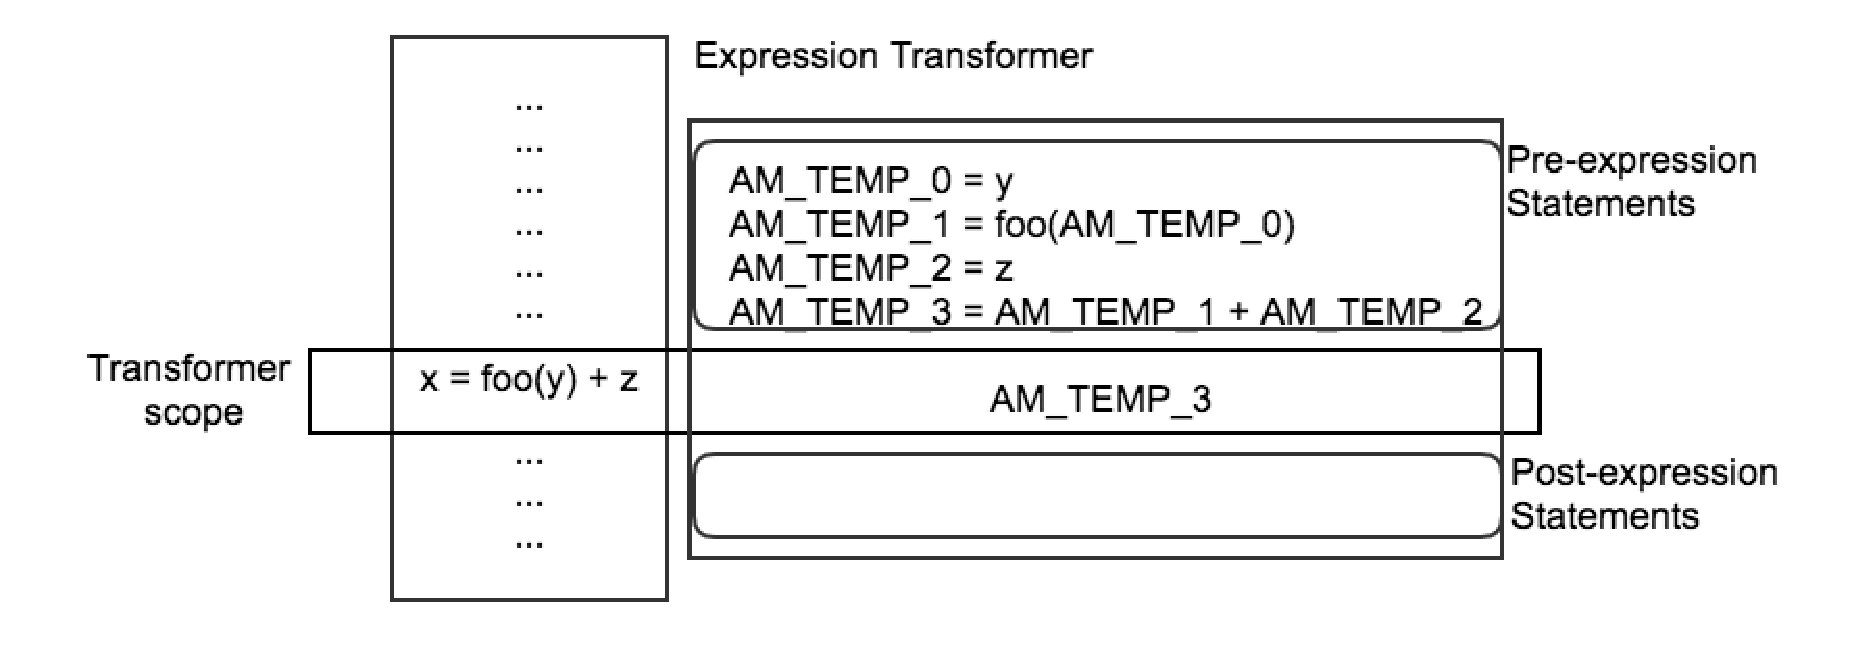
\includegraphics[width=0.9\textwidth]{figures/aspect_expr_transform}
    \end{center}
    \caption{Aspect Expression Transformer}
\end{figure}

\subsubsection{Statement Level Transformation}
The statement transformation is the second layer of the aspect transformation
framework. 
\begin{figure}[!htbp]
    \begin{center}
    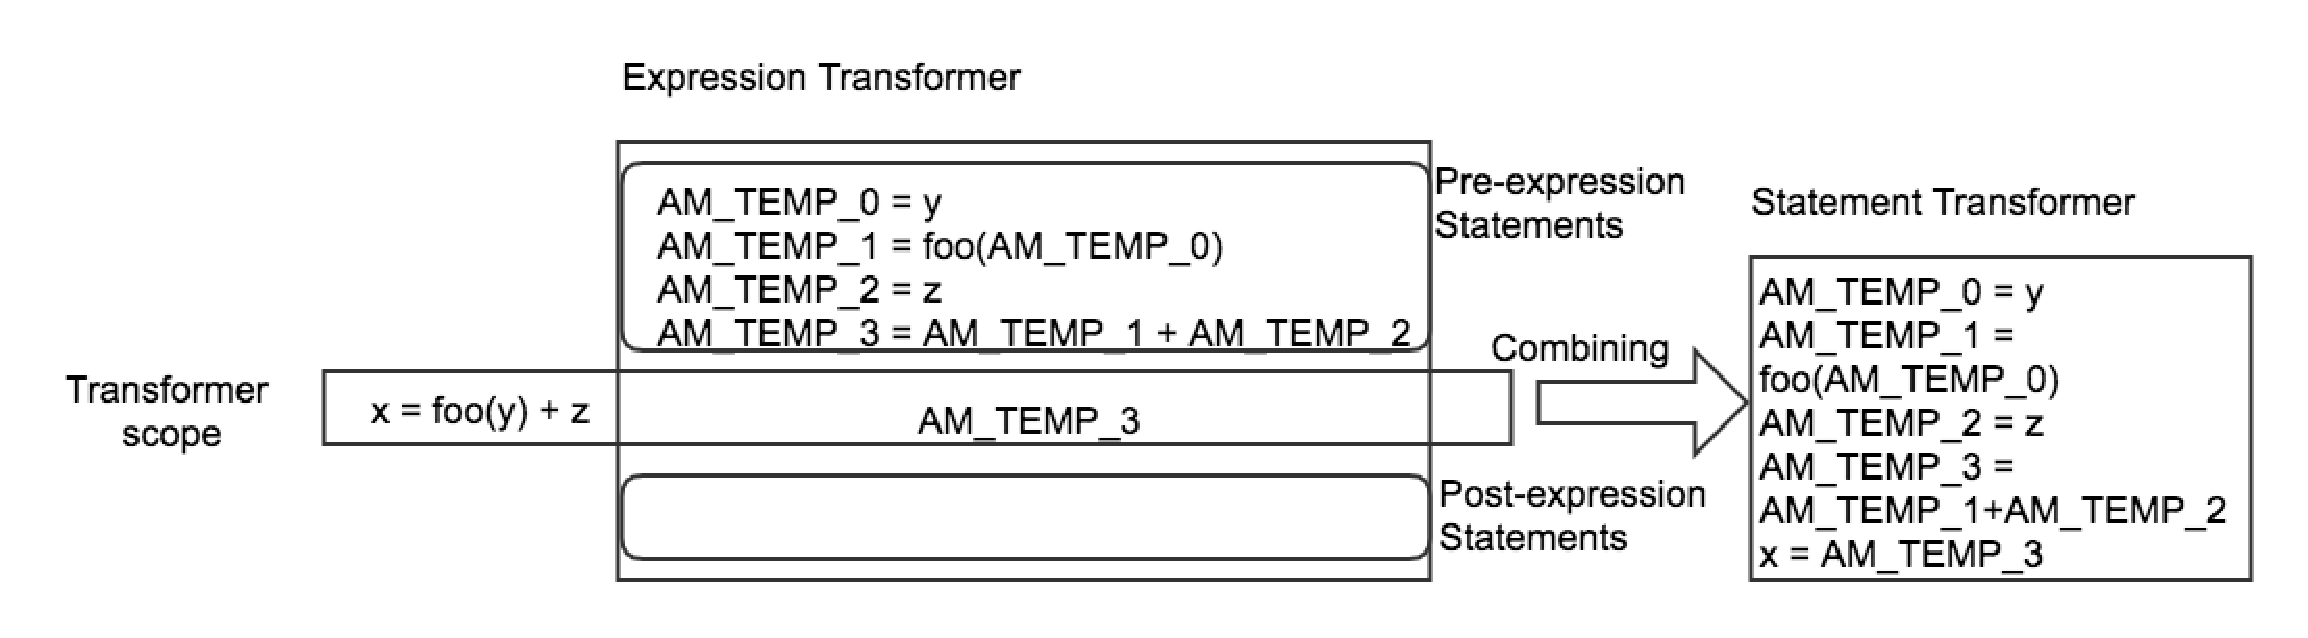
\includegraphics[width=0.9\textwidth]{figures/aspect_statement_transform}
    \end{center}
    \caption{Aspect Statement Transformer}
\end{figure}
It has two major responsibilities, the first one is to apply the
appropriate transformation to \emph{annotation}, \emph{loop}, \emph{loophead},
and \emph{loopbody} pattern. The second responsibility is to handle the
pre-expression statement and post-expression statement requests generated by
the expression transformer. As in the new transformation framework, the return
type of the statement transformation has been changed from void to
\emph{List$\langle$ast.Stmt$\rangle$}, the implementation of the statement
transformer is quite straight forward. The above diagram demonstrate the
process of a statement transformer.

\subsubsection{Program Level Transformation}
The program level transformation is the final piece in the aspect
transformation puzzle. Like statement level transformation it has two major
responsibilities - to handle the request generate by the statement level
transformation, and to apply appropriate transformation for the
\emph{execution} and \emph{mainexecution} pattern. After finish the
transformation, the program level transformer is also responsible to check the
validity of the transformed AST, for example, to make sure there do not exist a
self-loop within the AST. This make sure the transformation is robust, and
eliminate the possibility of unsound transformer implementation. Unlike the
previous version of transformation framework, we can implement these
parts modularly. This makes the compiler easy to maintain, and flexible for
further development.

\section{Conclusion}

In this project, we go over the details of implement an AspectMATLAB
front-end, and purpose a new modular transforming framework for more robust
transformation design. The new transformation framework split the whole
transformation process into three different parts, expression transformation,
statement transformation and program transformation. At each level, programmer
can focus on different aspect of design. The new transformation framework also
utilize the Java generic type-safe check mechanism. This make sure the
behaviour of the transformer is consistent (i.e. the in-place transformer will
also apply the transformation directly on the original AST, while the copy
transformer will return a copy of AST with modification applied).

\pagebreak
\appendix
\section{Links to Source Code and Toolkits}
\subsection{Andrew Bodzay's AspectMATLAB++ Compiler}
\url{https://github.com/Sable/AspectMatlab}
\subsection{New AspectMATLAB Compiler (Development)}
\url{https://github.com/Sable/AspectMATLAB-robust}
\subsection{McSAF (with updated parser and aspect AST Node)}
\url{https://github.com/Sable/mclab-parser}
\pagebreak

\bibliographystyle{plain}

\bibliography{bibliography}

\end{document}
